\section{Appendix}
\subsection{Broader Impact}
\label{app:impact}
This research contributes to the development of more efficient and reliable training protocols for LLMs specializing in complex reasoning. By introducing \method, we provide a mechanism to mitigate the risks of ``reward hacking'' and training instability inherent in dense on-policy distillation, where models might otherwise learn from low-quality or drifted teacher signals. The significant reduction in training compute (up to 68\%) directly addresses the environmental concerns associated with the high energy consumption of LLM post-training. By making sophisticated reasoning models more accessible to train with fewer resources, this work democratizes the ability to develop high-performing AI, potentially accelerating progress in scientific discovery.

Despite these benefits, we recognize that enhancing the reasoning capabilities of LLMs could inadvertently lower the barrier for generating sophisticated misinformation or dual-use content. While \method focuses on the process of learning rather than the content of the data, the resulting models could be more persuasive or harder to detect if used for deceptive purposes. To mitigate these risks, we emphasize the importance of using \method in conjunction with safety-aligned teacher models and rigorous verifiable RL frameworks. We are committed to transparency and reproducibility by providing detailed experimental setups and hyperparameter configurations, enabling the community to audit the reliability of these training dynamics and ensure that reasoning improvements do not come at the cost of model safety or ethical alignment.

\subsection{LLM Usage Declaration}
\label{app:llm_usage}
This manuscript uses LLMs strictly for the purpose of language editing and textual polishing to enhance presentation quality. We declare that the novel ideas, methodological framework, experimental execution, and data analysis are the original work of the authors. All content modified by AI tools has been carefully reviewed and validated by the authors to ensure accuracy.


\subsection{Limitations}

\method~relies on top-$k$ local-distribution statistics.
The primary overlap metric can miss cases where student and teacher share candidate tokens but rank or score them very differently, while the top-$p$ action-acceptance variant can be too strict for stylistically different but valid reasoning paths.
The current decay is linear in cumulative bad events and assumes that local compatibility correlates with reward exploitability; this can fail when a low-overlap prefix later returns to a teacher-compatible state.
The implementation also only rescales OPD rewards and does not attach a GRPO fallback to zero-reliability tokens.
Finally, the current experiments are limited to math reasoning with DeepSeek, Qwen, and Skywork-style models; agentic and multi-turn settings remain future work.

\subsection{Future Work}

A natural extension is to combine \method~with GRPO in a reliability-gated objective.
Before the reliability weight decays to zero, the model would still optimize the OPD loss and benefit from dense teacher guidance on locally compatible prefixes.
After the reliability weight reaches zero, the unreliable suffix would switch to a GRPO loss, allowing the student to continue exploring with outcome-level feedback instead of forcing it to follow a teacher distribution that is no longer locally exploitable.
Such a hybrid objective could combine the sample efficiency of teacher-guided distillation with the exploratory benefits of reinforcement learning, and may further improve long-horizon reasoning beyond reliability-aware truncation alone.



\subsection{Additional Related Work}
\label{app:related}
\paragraph{Knowledge distillation and off-policy distillation.}
Knowledge distillation transfers information from a teacher to a student by matching the teacher's soft output distribution \citep{hinton2015distilling}.
For autoregressive sequence models, sequence-level distillation trains the student on teacher-generated outputs \citep{kim2016sequence}, and this off-policy paradigm underlies many compact language-model distillation methods \citep{sanh2019distilbert,jiao2020tinybert,wang2020minilm,gu2026coevolvingpolicydistillation}.
Supervised fine-tuning and instruction tuning similarly improve downstream behavior by training on curated responses or demonstrations \citep{chung2024scaling,sanh2021multitask,wei2021finetuned}.
The common limitation is train-inference distribution mismatch: the student is optimized on teacher or reference trajectories, but at inference time it must condition on prefixes sampled from its own policy, an exposure-bias problem that compounds over long generations \citep{bengio2015scheduled}.
\method~follows the OPD motivation that distillation should be computed on student-visited states, but asks a further question: once the student is on-policy, which visited states still admit reliable dense teacher supervision?

\paragraph{OPD dynamics and mechanisms.}
Recent OPD analysis shows that OPD success is governed by thinking-pattern consistency and by whether the teacher contributes new knowledge beyond what the student has already acquired \citep{li2026rethinking}.
At the token level, successful OPD exhibits progressive alignment on high-probability tokens: top-$k$ overlap rises, overlap-token advantage improves, and the entropy gap narrows.
The same analysis further shows that reward quality degrades with trajectory depth, and that a reward can remain globally correlated with final correctness while failing to provide locally useful gradients around the student's current policy.
\method~directly operationalizes these diagnostic findings.
Instead of treating overlap ratio, entropy gap, or teacher acceptability as post-hoc measurements, it turns per-prefix compatibility into an online reliability signal that attenuates future OPD rewards and controls rollout length.

\paragraph{Capacity gap and distillability.}
A separate line of work studies when a teacher is too strong, too different, or too complex for the student to imitate.
% \citet{cho2019efficacy} show that overly capable teachers can hurt student performance, and \citet{mirzadeh2020improved} introduce teacher assistants to bridge large capacity gaps.
Studies have shown that overly capable teachers can hurt student performance \citep{cho2019efficacy}, and teacher assistants have been introduced to bridge large capacity gaps \citep{mirzadeh2020improved}.
Distillation scaling laws identify non-monotonic interactions among teacher quality, student size, and data volume \citep{busbridge2025distillation}.
For reasoning models, small students can struggle to learn from strong reasoners with long chain-of-thought traces, suggesting a learnability gap in distilling complex reasoning behavior \citep{li2025small}.
These results caution against assuming that teacher benchmark strength alone determines distillation quality.
\method~studies the same issue from an on-policy, position-wise perspective: a teacher may be useful globally but unreliable at specific depths of a student-generated trajectory.


\noindent\textbf{Reasoning RL and long-horizon supervision.}
Modern reasoning models rely on verifiable RL, long chain-of-thought rollouts, and large mathematical training sets \citep{shao2024deepseekmath,guo2025deepseek,yu2025dapo,he2025justrl,accordion,dars,yang2025optibench,xu2026envfactoryscalingtooluseagents}.
Long responses create room for search and self-correction, but they also make dense supervision expensive and harder to trust.
Prior OPD results identify a response-length sweet spot: short responses provide too little dense signal, while very long responses can trigger late-stage collapse and suffix-to-prefix instability \citep{li2026rethinking}.
\method~is designed for this long-horizon setting.
It does not impose a fixed response budget; it estimates which prefixes still carry reliable teacher signal and uses that estimate for both reward scaling and dynamic response-length control.

\subsection{Reliability Rationale}
\label{app:rationale}

\method~is motivated by the distinction between globally informative teacher rewards and locally exploitable token-level supervision on student-visited prefixes~\citep{li2026rethinking}.
Overlap ratio and related compatibility metrics are therefore used online: repeated low-compatibility events are treated as evidence that the student trajectory has drifted into a region where uniform dense OPD rewards are less trustworthy.
The method does not assume that every low-overlap token is wrong; it only assumes that cumulative compatibility failure is a useful path-dependent signal for attenuating later suffix rewards.

The monotone reliability decay is a deliberately conservative design.
Later tokens can become locally compatible because the teacher adapts to an already drifted prefix, not because the full reasoning trajectory has returned to a teacher-compatible state.
Using cumulative decay avoids re-amplifying suffix rewards after repeated drift events, while the base weight $w_{\mathrm{base}}$ separates the reliability estimate $R_{\tau}$ from the optimization scale $L_{\tau}$.
This lets \method~down-weight unreliable suffix supervision without turning the method into a brittle hard filter.


\subsection{Implementation Details}

\method~is implemented as a post-processing step on the \opd~reward tensor.
The baseline reward tensor has shape $[B,T,k]$, where $B$ is batch size, $T$ is response length, and $k$ is the top-$k$ token dimension.
For each valid response position, the method computes the scalar loss weight $L_{\tau}$ and multiplies every candidate reward at that position by the same scalar:
\begin{equation}
    \widetilde{r}_{b,\tau,j}=L_{b,\tau}r_{b,\tau,j}.
\end{equation}
Padding positions have $R_{\tau}=0$ and $L_{\tau}=0$.
The advantage estimator remains \texttt{token\_reward\_direct}, so the scaled reward is used directly as the token-level advantage.

The current code path keeps the baseline isolated.
When \texttt{prune\_opd.enable=False}, the original \opd/\grpo behavior is unchanged.
When enabled, the main experiments use \texttt{overlap\_ratio}; \texttt{teacher\_top\_p\_accept} is retained as an action-level variant.
The teacher top-$k$ size is controlled by \texttt{actor\_rollout\_ref.rollout.log\_prob\_top\_k} and is set to 16 in the current experiments.


\subsection{Prompt Template}
\label{app:prompt-template}

We use the same DAPO-Math prompt template as the OPD dynamics study~\citep{li2026rethinking}.
For each math problem, the raw question is inserted into the following instruction.

\definecolor{promptboxbg}{HTML}{F2E9FF}
\definecolor{promptboxframe}{HTML}{7E57C2}
\begin{center}
\setlength{\fboxsep}{8pt}
\fcolorbox{promptboxframe}{promptboxbg}{%
\begin{minipage}{0.92\linewidth}
\textbf{DAPO-Math Prompt Template}\\[0.35em]
\small
\{Question\} Please reason step by step, and put your final answer within \textbackslash boxed\{\}.
\end{minipage}}
\end{center}

\subsection{Primary Configurations}
Table~\ref{tab:hyperparams} summarizes the primary hyperparameters used across our \method~experiments.
Unless otherwise stated, all benchmark performance reported in the paper is Avg@16 accuracy: for each benchmark problem, evaluation uses 16 sampled responses under the fixed evaluation protocol and reports the average correctness across those samples. For high compatibility pair (DeepSeek-R1-Distill-Qwen-7B / Skywork-OR1-7), the init dynamic length is set as 6144; For other pairs, the init dynamic length is set as 1024.

\begin{table}[h]
\centering
\caption{\textbf{Default hyperparameters for \method.}}
\label{tab:hyperparams}
\small
\begin{tabular}{lc}
\toprule
\textbf{Item} & \textbf{Value} \\
\midrule
Training dataset & DAPO-Math-17K \\
Training temperature & 1.0 \\
Teacher temperature & 1.0 \\
Rollout number & 4 \\
Mini batch size & 64 \\
LogProb top-$K$ & 16 \\
Top-$K$ strategy & Student Top-$K$ \\
Reward weight mode & Student probability \\
Max prompt length & 1,024 \\
Max response length & 8,192--12,288 \\
Validation max response length & 31,744 \\
Learning rate & $1\times10^{-6}$ \\
Training steps & 203 \\
KL coefficient & 0.0 \\
Loss aggregation & \texttt{token-mean} \\
Overlap threshold $\gamma$ & 0.7 \\
Top-$p$ threshold $p$ & 0.95 \\
$w_{\mathrm{drop}}$ & 0.01 \\
$w_{\mathrm{base}}$ & 0.5 \\
Dynamic length init/min/max & 1024 / 1024 / 12288 \\
Dynamic length step & 100 \\
Hit ratio threshold & 0.1 \\
Length margin & 100 \\
Shrink patience & 3 \\
\bottomrule
\end{tabular}
\end{table}



\subsection{Top-$p$ Action-Acceptance Metric}
\label{app:top-p-metric}

In addition to overlap ratio, we evaluate a stricter action-level compatibility metric.
At position $\tau$, the student samples the actual next token $y_{\tau}$, while the teacher returns top-$k$ tokens and probabilities under the same prefix:
\begin{equation}
    \topk = \{v_{\tau,1}, \ldots, v_{\tau,k}\}, \qquad
    q_{\tau,1} \geq q_{\tau,2} \geq \cdots \geq q_{\tau,k}.
\end{equation}
Given a top-$p$ threshold $p$, define the cumulative visible mass
\begin{equation}
    S_{\tau,m} = \sum_{j=1}^{m} q_{\tau,j}.
\end{equation}
If a smallest $m_{\tau}$ satisfies $S_{\tau,m_{\tau}}\geq p$, the visible nucleus is
\begin{equation}
    \accept(p,k)=\{v_{\tau,1},\ldots,v_{\tau,m_{\tau}}\}.
\end{equation}
If the returned top-$k$ mass is still below $p$, the true nucleus extends beyond the observed set, so we conservatively use $\accept(p,k)=\topk$.
The bad event is $B_{\tau}=\mathbf{1}[y_{\tau}\notin\accept(p,k)]$.
In the reported top-$p$ runs, $p=0.95$.





\subsection{Why \method Can Improve Accuracy for Low-Overlap Qwen Pairs?}
\label{app:qwen-low-overlap}

Table~\ref{tab:main-results} shows that the two Qwen3 teacher-student pairs, Qwen3-1.7B-Base / Qwen3-4B (Non-thinking) and Qwen3-4B-Base / Qwen3-4B (Non-thinking), are the clearest cases where \method~improves both training efficiency and benchmark accuracy.
We interpret this as a low-overlap regime where reliability-aware pruning acts not only as a compute-saving mechanism, but also as a gradient denoising mechanism.
As shown in Figure~\ref{fig:appendix-qwen-short-effective-length}, these pairs exhibit low student-teacher overlap, and \method~therefore keeps the effective OPD length at only a few hundred tokens.
In contrast, the corresponding OPD baseline uses a maximum response budget of 12,288 tokens.

This mismatch creates a plausible failure mode for unpruned OPD.
Only the early prefix contains locally exploitable teacher supervision, while the long suffix contributes a large number of token-level gradients produced on drifted, low-overlap prefixes.
Because those suffix tokens vastly outnumber the useful prefix tokens, their gradients can dominate the update even if each individual suffix reward is weak or noisy.
\method~removes this imbalance by attenuating and truncating low-reliability suffixes, concentrating optimization on the short prefix where the teacher remains actionable.
This explains why these two Qwen3 pairs can gain accuracy in addition to saving time.
For the other teacher-student combinations, compatibility is higher or the useful supervision window is already long enough that pruning mainly reduces computation while preserving accuracy, rather than substantially changing the effective training signal.

\begin{figure*}[t]
\centering
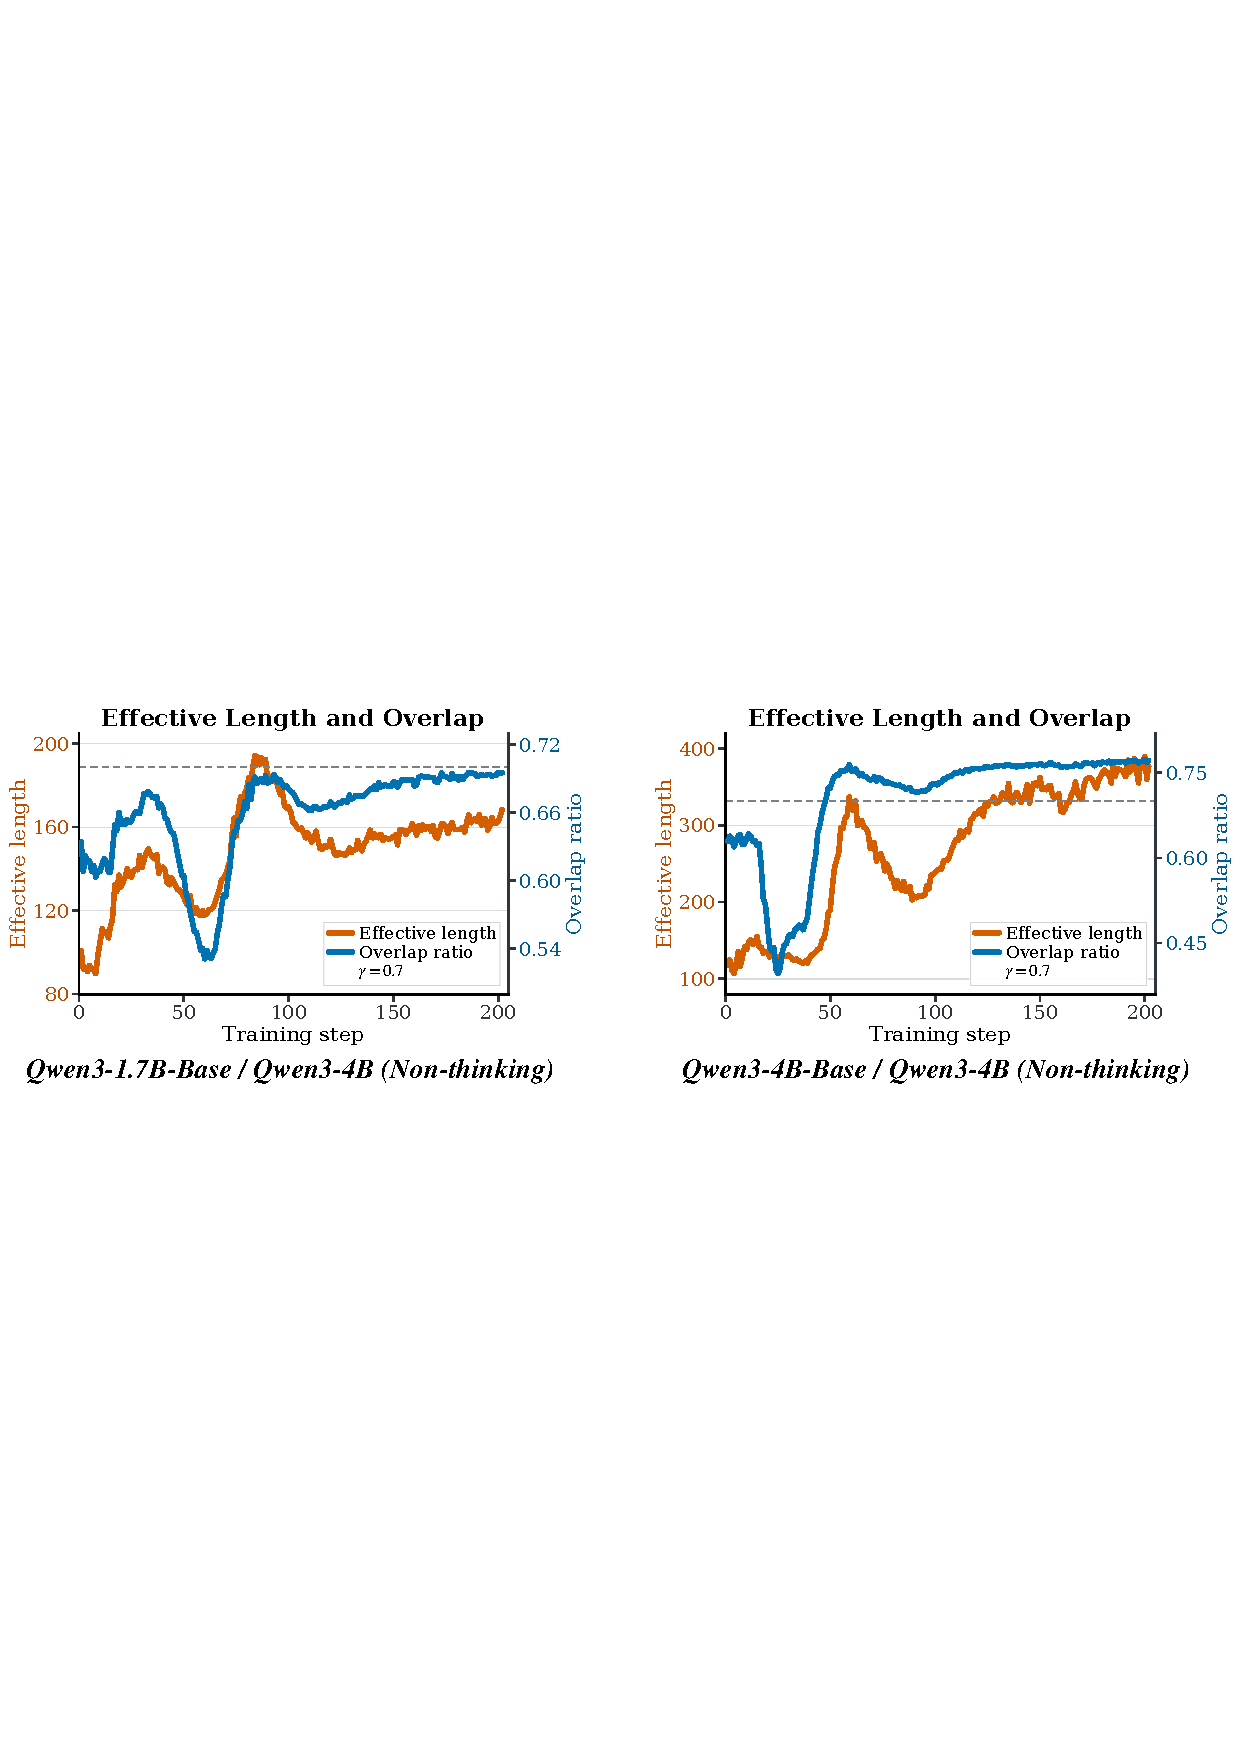
\includegraphics[width=\textwidth]{figs/apd-short_compat.pdf}
\caption{Short effective OPD windows in the low-overlap Qwen3 distillation pairs. For Qwen3-1.7B-Base / Qwen3-4B (Non-thinking) and Qwen3-4B-Base / Qwen3-4B (Non-thinking), low overlap causes \method~to concentrate OPD supervision within a few hundred reliable tokens, whereas the OPD baseline keeps training on responses up to 12,288 tokens.}
\label{fig:appendix-qwen-short-effective-length}
\end{figure*}



\subsection{Additional Diagnostics}

The appendix diagnostics focus on the compatibility signals that motivate \method.
Figure~\ref{fig:appendix-opd-overlap-dynamics} reports how overlap ratio evolves across depth bands under unpruned OPD, and Figure~\ref{fig:appendix-threshold-diagnostics} shows how the overlap threshold controls suffix down-weighting and the dynamic response budget.

\paragraph{Depth-wise overlap under OPD.}
Figure~\ref{fig:appendix-opd-overlap-dynamics} isolates the compatibility dynamics of the unpruned OPD baseline.
The shallow 0--1K band acts as a reference for early-prefix supervision, while the later bands test whether teacher supervision remains locally aligned after long student-generated reasoning prefixes.
The key observation is that compatibility is depth-dependent: later token-position bands are the regime where overlap is most fragile and where uniform dense rewards are least likely to provide useful local gradients.
This supports the central premise of \method: the inefficiency of long-horizon OPD is not only that suffixes are expensive, but that the suffix rewards are often produced on prefixes where the teacher and student have already drifted apart.

\begin{figure*}[t]
\centering
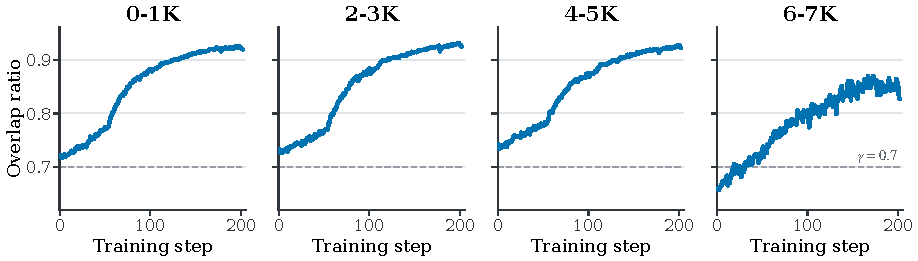
\includegraphics[width=\textwidth]{figs/fig7_opd_overlap_four_panels.pdf}
\caption{OPD baseline overlap-ratio training dynamics for DeepSeek-R1-Distill-Qwen-1.5B / JustRL-DeepSeek-1.5B. Each panel plots overlap ratio versus training step for a token-position band: 0--1K, 2--3K, 4--6K, and 7--8K. This diagnostic shows how local student-teacher compatibility evolves at different trajectory depths under unpruned OPD.}
\label{fig:appendix-opd-overlap-dynamics}
\end{figure*}

\paragraph{Threshold sensitivity.}
Figure~\ref{fig:appendix-threshold-diagnostics} explains how the reliability threshold changes the intervention.
A larger threshold declares compatibility failures earlier, which makes the token-level weight decay sooner and yields a shorter dynamic OPD budget; a smaller threshold is more permissive and preserves longer suffix supervision.
The main setting $\gamma=0.7$ lies between these extremes: it removes a substantial amount of low-reliability suffix computation while avoiding the overly rigid behavior of a hard fixed-length truncation.
Thus the threshold primarily controls where \method~sits on the reliability--compute axis, rather than changing the underlying OPD objective.

\begin{figure*}[t]
\centering
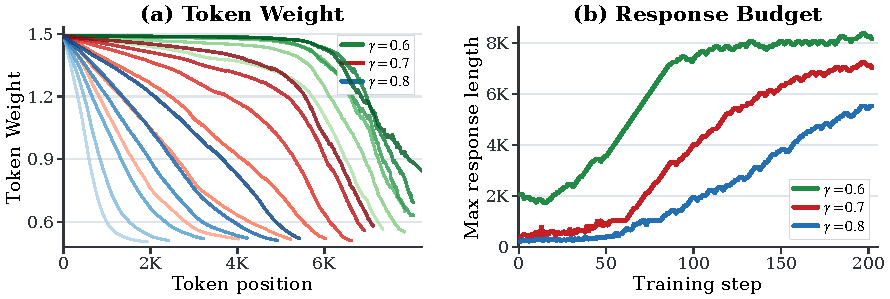
\includegraphics[width=\textwidth]{figs/fig8_threshold_diagnostics.pdf}
\caption{Prune-OPD threshold diagnostics for DeepSeek-R1-Distill-Qwen-1.5B / JustRL-DeepSeek-1.5B. Left: mean Prune-OPD weight as a function of token position under three overlap thresholds, $\gamma=0.6,0.7,0.8$; for each threshold, the curves are taken at training steps 100, 120, 140, 160, 180, and 200. Right: maximum OPD response length over training steps under the same thresholds. Together, these diagnostics show how the reliability threshold changes suffix down-weighting and dynamic rollout budgets.}
\label{fig:appendix-threshold-diagnostics}
\end{figure*}


\subsection{Compute Reporting}
\label{app:compute-reporting}

The dominant compute cost comes of our work from post-training student models with OPD-style teacher scoring and from benchmark evaluation.
For each teacher-student pair, OPD, fixed truncation, and \method~are run under the same training stack and matched hardware allocation, so the reported wall-clock comparisons isolate the effect of reliability-aware pruning rather than changes in infrastructure.
The main compute evidence is therefore reported as elapsed training time in Tables~\ref{tab:main-results}, \ref{tab:high-compatibility}, and \ref{tab:threshold-ablation}, and in Figure~\ref{fig:time-accuracy}